
\subsection{Stormfloder} \label{Afsnit: Stormfloder}

En stormflod er betegnelsen for usædvanligt højvande i relation til kraftig vind \citep{shoreline_management_guidelines}. En stormflod bliver dannet og påvirkes af fire primære drivkræfter. Vindstuvning der presser havvand mod kysten, imod landmassen, bølgepåvirkning der kan intensivere denne effekt, et lavere tryk vil hæve vandstandsniveau lokalt og hvis vandstanden sker i et område med tidevand kan vandstanden stige markant under højvande \citep{piecuch_high-tide_2022}.
Styrken og påvirkningen af en stormflod på en lokalitet er afhængig af en række faktorer herunder orienteringen af kysten i forhold til stormen, hvor kraftig stormen er og de lokale havbunds- og dybdeforhold \citep{noaa_storm, shoreline_management_guidelines}. \\

I Danmark er det Vadehavskysten der ofte er det mest udsatte område, da vinden i Danmark primært kommer fra vest \citep{cappelen_dmi_2020}. Over længere perioder med vesten vind, vil vandet i Nordsøen blive presset ind Kattegat og længere ned i de indre danske farvande. Hvis vinden er langvarig, vil vandet over tid blive presset igennem bælterne ved Lillebælt, Storebælt og Øresund og videre ind i Østersøen og nord imod den Botniske Bugt \citep{kiesel_brief_2024, egusphere_baltic}. Dette fænomen kaldes for \textit{"preconditioning"} og beskriver hvordan vandstanden stiger i Østersøen inden begyndelsen af en storm \citep{kiesel_brief_2024, weisse_sea_2021}. \\   

Når vinden derefter aftager eller ændrer retning vil alt vandet der er blevet presset ind i Østersøen, skvulpe tilbage mod bælterne i Danmark. Dette kaldes for \textit{"badekarseffekten"} og er illustreret i figur \ref{Figur: Bathtub effect} \citep{kystdirektoratet_stormfloder, egusphere_baltic}. Bælterne i de indre danske farvande vil herefter fungere som flaskehalse for vandmasserne der skvulper tilbage fra Østersøen og resultere i oversvømmelse i de indre danske farvande \citep{egusphere_baltic}.
\begin{figure}[H]
    \centering
    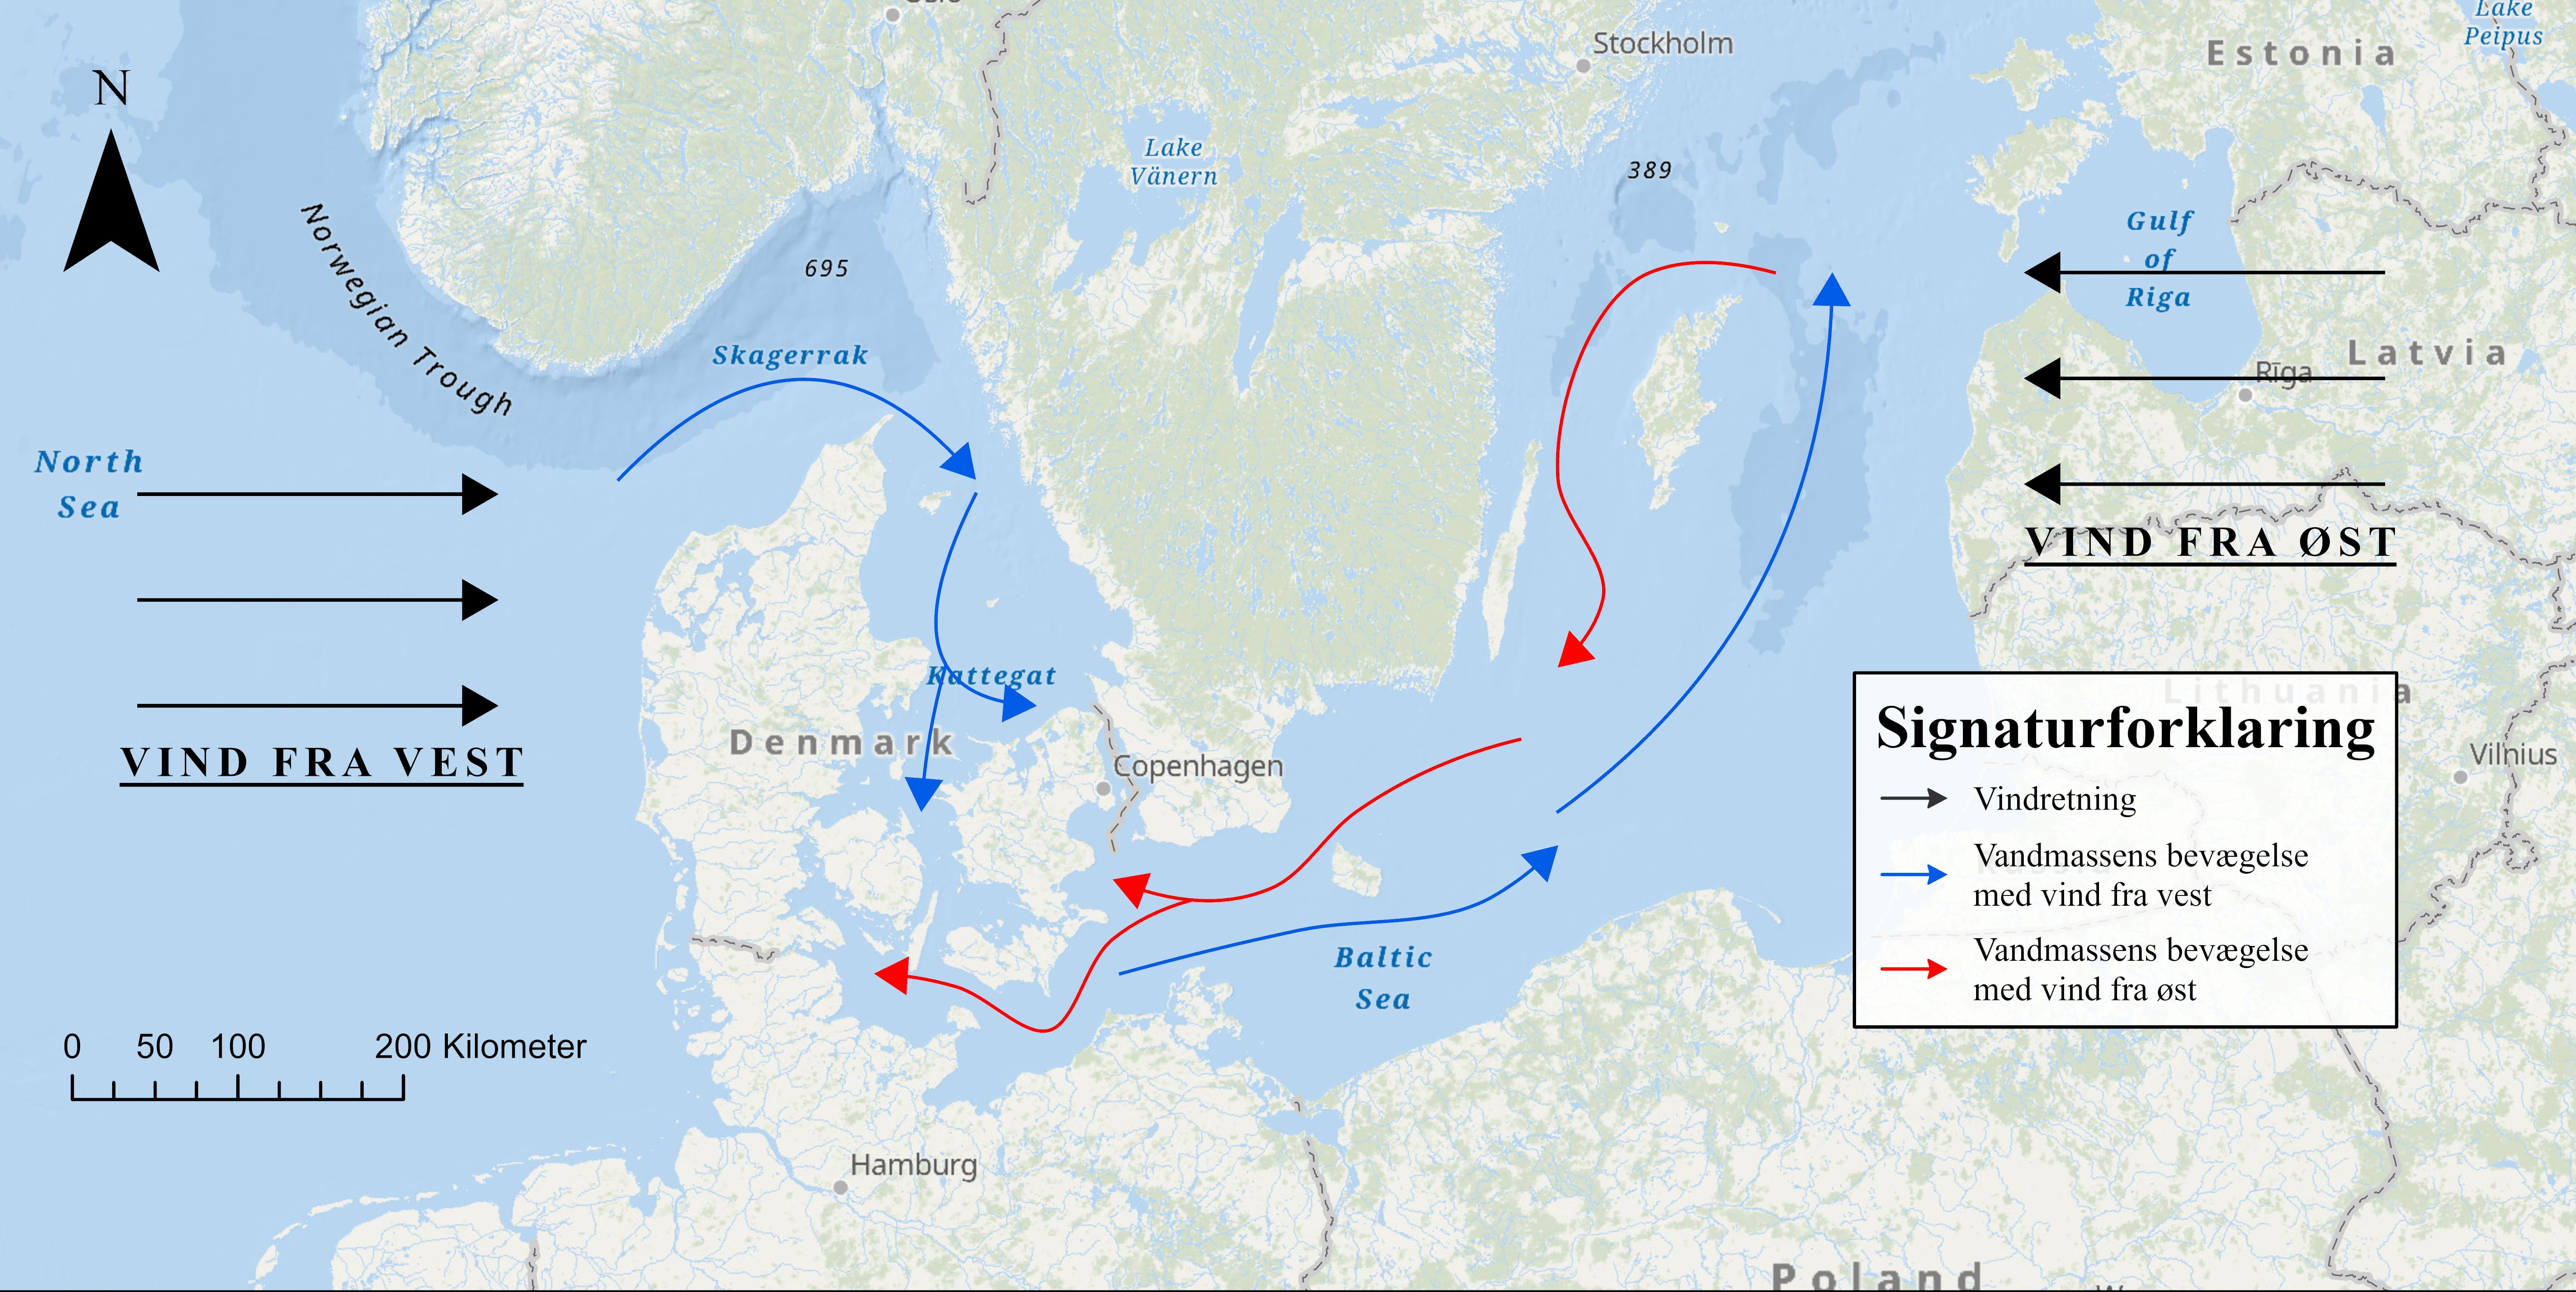
\includegraphics[width=0.8\linewidth]{images/teori/bathtub effect graphics.jpg}
    \caption{Illustration af "badekarseffekten". De sorte pile indikerer vindretning og de blå og røde pile indikerer bevægelsen af vandmassen. Kilde: Egen illustration, baggrundskort fra Esri}
    \label{Figur: Bathtub effect}
\end{figure}
Nævneværdige stormfloder som stormfloden den 1.-2. november 2006, den 20.-21. oktober 2023 og den 12.-14. november 1872 blev forårsaget af en kraftig østenvind efter længerevarende vestenvind og \textit{"badekarseffekten"} \citep{kystdirektoratet_stormfloder}.

\subsection{Stormfloden den 20 oktober 2023} \label{Afsnit: Stormfloden den 20 oktober 2023}
I første halvdel af oktober 2023 blev der observeret moderate vindforhold med gennemsnitlig middelvind på 5,5 m/s og en gennemsnitlig maksimal 10.min middelvind på 18,3 m/s fra vest, hvilket medførte en betydelig vandtransport ind gennem Kattegat og videre i Østersøen \citep{dmi_vejrarkiv}. \\
Den 18. oktober skiftede vindretningen til øst (figur \ref{Figur: Vinddata Danmark}) grundet trykforskelle mellem et højtryksystem over Skandinavien og et lavtrykssystem over Storbritannien \citep{kiesel_brief_2024}, og middelvindhastigheden steg i hele landet til 12,2 m/s og maksimale 10.min middelvind til 28,3 m/s om aftenen den 20. oktober 2023. 
\begin{figure} [H]
    \centering
    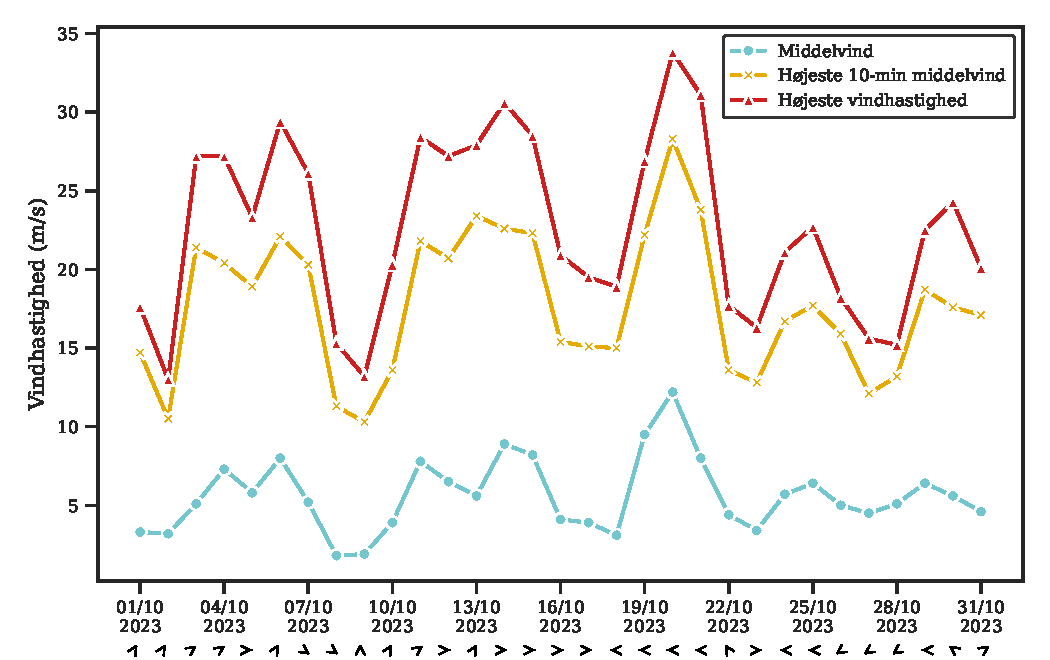
\includegraphics[width=0.8\linewidth]{images/teori/vinddata_grafer/Danmark_vinddata.pdf}
    \caption{Vinddata for Danmark i oktober 2023 der viser middelvind, højeste 10.min middelvind og højeste vindhastighed i m/s. De sorte pile i bunden indikerer vindretningen. Kilde: Data fra \cite{dmi_vejrarkiv} }
    \label{Figur: Vinddata Danmark}
\end{figure}

Kombinationen af kraftig vind fra øst og stor vandtransport ind i Østersøen over en periode på 15 dage resulterede ifølge \cite{kystdirektoratet_stormflod2023} i markante vandstandsstigninger i de indre farvande af Syddanmark i løbet af eftermiddagen den 20. oktober. Den højeste officielle vandstand målt under stormfloden blev målt i Aabenraa Havn på 2,16 m over dagligt vande \citep{damberg_vaerste_2023}. Disse forhold forårsagede omfattende skader af sommerhusområder, kystnære områder og byer \citep{kystdirektoratet_stormflod2023, naturskaderadet_anmeldelser_2023}. 




